% 18 variables in here:
% h_1 = 10.0, h_2 = 10.0, h_3 = 10.0, h_4 = 10.0, h_5 = 10.0, h_6 = 10.0, ux_1 = 0.0, ux_2 = 0.0, ux_3 = 0.0, ux_4 = 0.0, ux_5 = 0.0, ux_6 = 0.0, uy_1 = 0.0, uy_2 = 0.0, uy_3 = 0.0, uy_4 = 0.0, uy_5 = 0.0, uy_6 = 0.0
\begin{figure}[ht!]
\centering
  \subfigure[$SE^1_x$, $SE^1_y$] {
    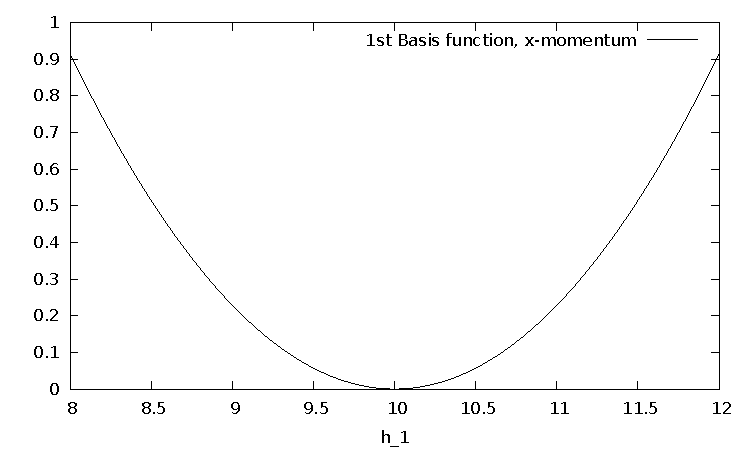
\includegraphics[scale=\zoomfactor]{{{ord2_varying_h1_default/y_10.0_10.0_10.0_10.0_10.0_0.0_0.0_0.0_0.0_0.0_0.0_0.0_0.0_0.0_0.0_0.0_0.0f00}}}
  }
  % \subfigure[] {
  %   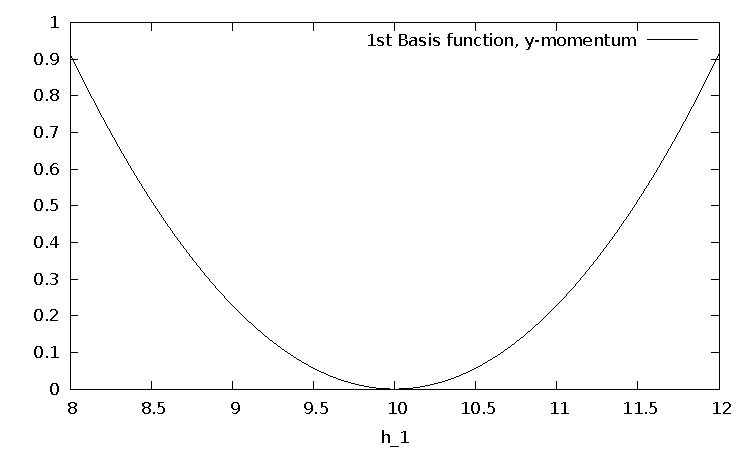
\includegraphics[scale=\zoomfactor]{{{ord2_varying_h1_default/y_10.0_10.0_10.0_10.0_10.0_0.0_0.0_0.0_0.0_0.0_0.0_0.0_0.0_0.0_0.0_0.0_0.0f01}}}
  % }
  \subfigure[$SE^2_x$, $SE^6_y$] {
    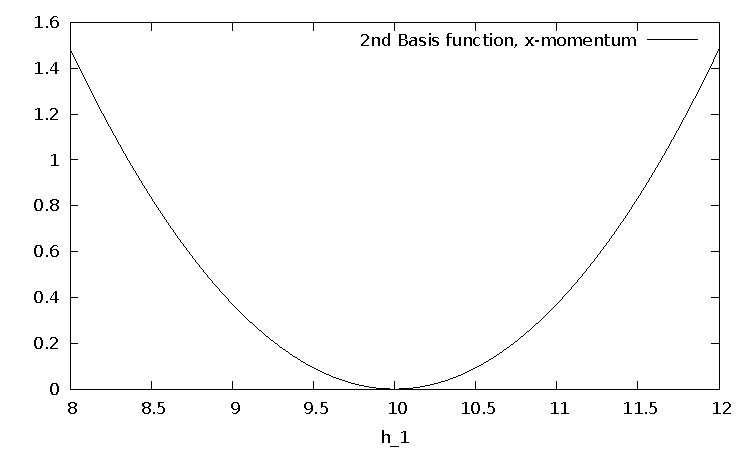
\includegraphics[scale=\zoomfactor]{{{ord2_varying_h1_default/y_10.0_10.0_10.0_10.0_10.0_0.0_0.0_0.0_0.0_0.0_0.0_0.0_0.0_0.0_0.0_0.0_0.0f02}}}
  }
  \subfigure[$SE^2_y$, $SE^4_x$, $SE^4_y$, $SE^6_x$] {
    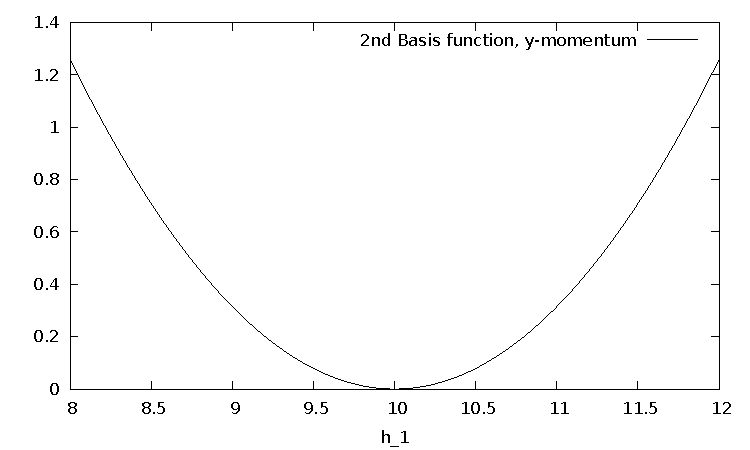
\includegraphics[scale=\zoomfactor]{{{ord2_varying_h1_default/y_10.0_10.0_10.0_10.0_10.0_0.0_0.0_0.0_0.0_0.0_0.0_0.0_0.0_0.0_0.0_0.0_0.0f03}}}
  }
  \subfigure[$SE^3_x$, $SE^5_y$] {
    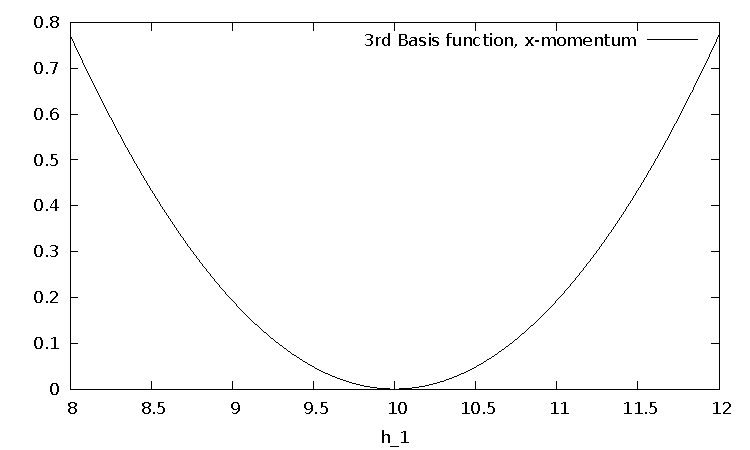
\includegraphics[scale=\zoomfactor]{{{ord2_varying_h1_default/y_10.0_10.0_10.0_10.0_10.0_0.0_0.0_0.0_0.0_0.0_0.0_0.0_0.0_0.0_0.0_0.0_0.0f04}}}
  }
  % \subfigure[3rd basis function, $y$-momentum -- 5th basis function, $x$-momentum] {
  %   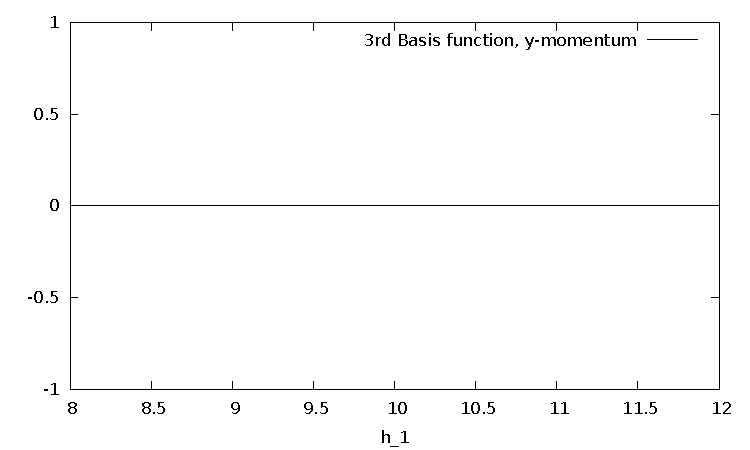
\includegraphics[scale=\zoomfactor]{{{ord2_varying_h1_default/y_10.0_10.0_10.0_10.0_10.0_0.0_0.0_0.0_0.0_0.0_0.0_0.0_0.0_0.0_0.0_0.0_0.0f05}}}
  % }
  % \subfigure[] {
  %   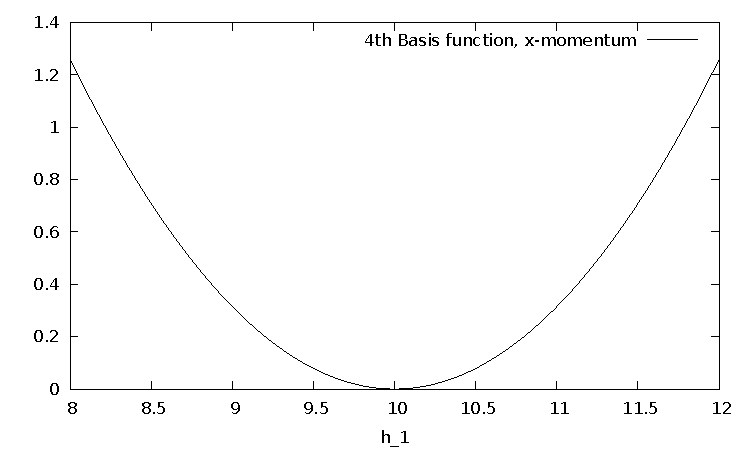
\includegraphics[scale=\zoomfactor]{{{ord2_varying_h1_default/y_10.0_10.0_10.0_10.0_10.0_0.0_0.0_0.0_0.0_0.0_0.0_0.0_0.0_0.0_0.0_0.0_0.0f06}}}
  % }
  % \subfigure[] {
  %   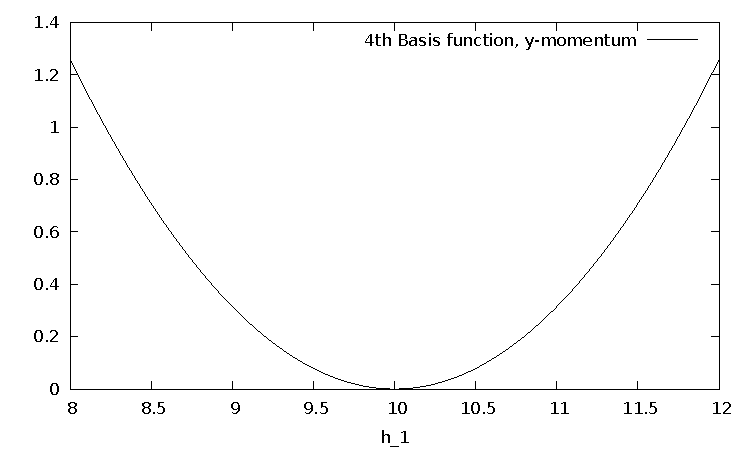
\includegraphics[scale=\zoomfactor]{{{ord2_varying_h1_default/y_10.0_10.0_10.0_10.0_10.0_0.0_0.0_0.0_0.0_0.0_0.0_0.0_0.0_0.0_0.0_0.0_0.0f07}}}
  % }
  % \subfigure[] {
  %   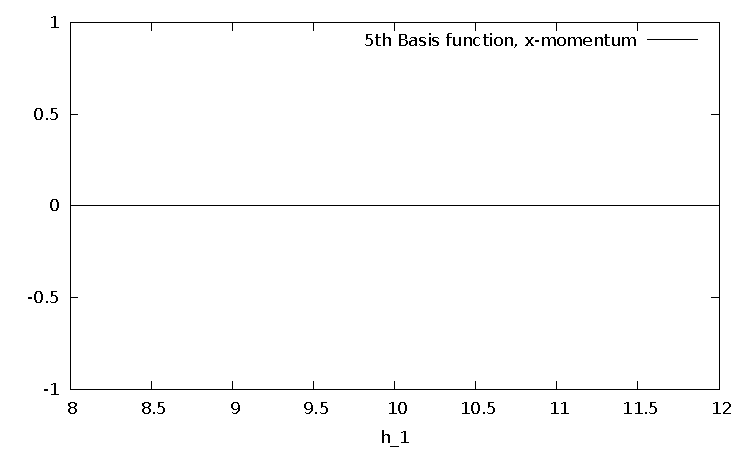
\includegraphics[scale=\zoomfactor]{{{ord2_varying_h1_default/y_10.0_10.0_10.0_10.0_10.0_0.0_0.0_0.0_0.0_0.0_0.0_0.0_0.0_0.0_0.0_0.0_0.0f08}}}
  % }
  % \subfigure[] {
  %   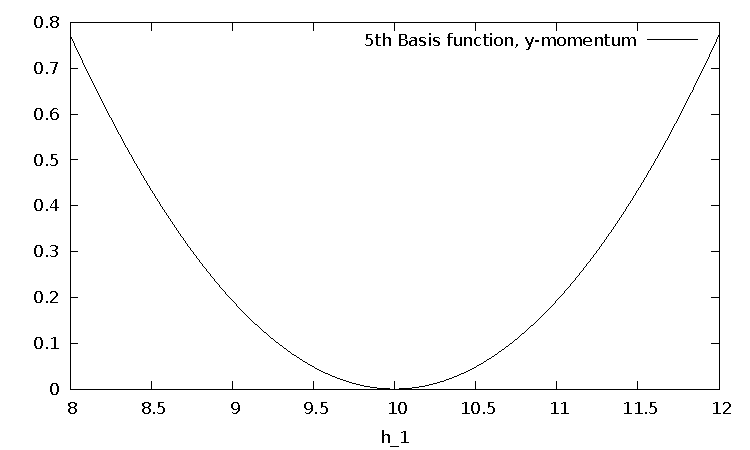
\includegraphics[scale=\zoomfactor]{{{ord2_varying_h1_default/y_10.0_10.0_10.0_10.0_10.0_0.0_0.0_0.0_0.0_0.0_0.0_0.0_0.0_0.0_0.0_0.0_0.0f09}}}
  % }
  % \subfigure[] {
  %   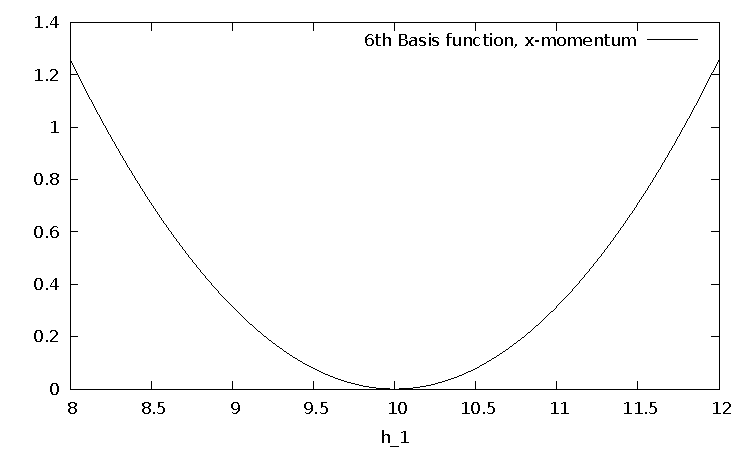
\includegraphics[scale=\zoomfactor]{{{ord2_varying_h1_default/y_10.0_10.0_10.0_10.0_10.0_0.0_0.0_0.0_0.0_0.0_0.0_0.0_0.0_0.0_0.0_0.0_0.0f10}}}
  % }
  % \subfigure[] {
  %   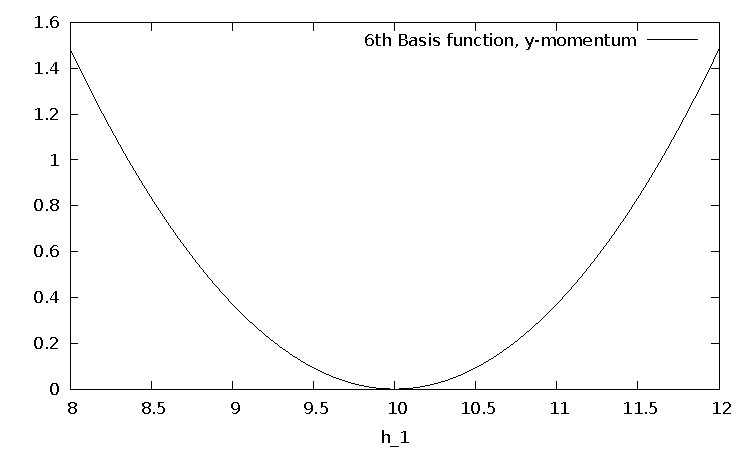
\includegraphics[scale=\zoomfactor]{{{ord2_varying_h1_default/y_10.0_10.0_10.0_10.0_10.0_0.0_0.0_0.0_0.0_0.0_0.0_0.0_0.0_0.0_0.0_0.0_0.0f11}}}
  % }
\caption{Error plots for varying $h_1$. All heights are fixed to 10 (except, of course, $h_1$) and all momentums are 0. The errors for the $y$-momentum of the 3rd basis function and the $x$-momentum for the 5th basis function are 0.}
\label{fig:ord2_varying_h1_default}
\end{figure}

%%% Local Variables:
%%% TeX-master: "../results.tex"
%%% End:
